

\documentclass{article}
\usepackage[english]{babel}
\usepackage[utf8]{inputenc}
\usepackage{fancyhdr}
\usepackage[export]{adjustbox}
 
\pagestyle{fancy}
\fancyhf{}
\rhead{Ricardo Nunes}
\lhead{Homework 7}
\rfoot{Page \thepage}
 
\begin{document} 
\paragraph{A.1}  --------\\
	\(\textbf{a)}\) big = 3\\ 
	\(\textbf{b)}\) 2 swaps. One between numbers 2 and 4 and the last between 3 and 1. \\ 
	\(\textbf{c)}\) \([1,1,2,3,5,9,4,6]\)\\
	\(\textbf{d)}\) \(sort(0,2)\) will in its recursive call have a \(k =  split(0, 2) = 1\). For the other half \(sort(4,7)\) will in its recursion have \(k = split(4, 7) = 5\);\\
	
\paragraph{A.2} --------\\
\begin{figure}[h]
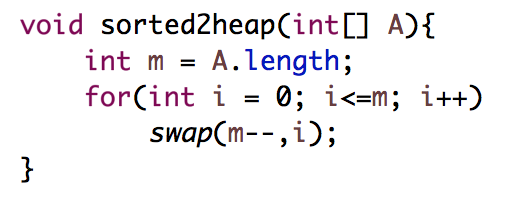
\includegraphics[width=0.5\textwidth, inner]{Hw7fig}
\end{figure}
 
 
 \paragraph{A.3} --------\\
 \\\(\textbf{(i)}\)  The worst case will be for a list with reversed order of elements. \\  \\
	And argue why it has \(\ghama(n2)\) comparisons.  
	\\ \\ \\ 
 \\\[\textbf{(ii)}\)
  \begin{tabular}{ccc}
  10, 9, 8, 7, 6, 5, 4, 3, 2, 1 &  4, 5, 6, 7, 8, 9, 3, 10, 2, 1 \\
  9, 10, 8, 7, 6, 5, 4, 3, 2, 1 &  4, 5, 6, 7, 8, 3, 9, 10, 2, 1 \\
  9, 8, 10, 7, 6, 5, 4, 3, 2, 1 &  4, 5, 6, 7, 3, 8, 9, 10, 2, 1 \\
  8, 9, 10, 7, 6, 5, 4, 3, 2, 1 &  4, 5, 6, 3, 7, 8, 9, 10, 2, 1 \\
  8, 9, 7, 10, 6, 5, 4, 3, 2, 1 &  4, 5, 3, 6, 7, 8, 9, 10, 2, 1 \\
  8, 7, 9, 10, 6, 5, 4, 3, 2, 1 &  4, 3, 5, 6, 7, 8, 9, 10, 2, 1 \\
  7, 8, 9, 10, 6, 5, 4, 3, 2, 1 &  3, 4, 5, 6, 7, 8, 9, 10, 2, 1 \\ 
  7, 8, 9, 6, 10, 5, 4, 3, 2, 1 &  3, 4, 5, 6, 7, 8, 9, 2, 10, 1 \\
  7, 8, 6, 9, 10, 5, 4, 3, 2, 1 &  3, 4, 5, 6, 7, 8, 2, 9, 10, 1 \\
  7, 6, 8, 9, 10, 5, 4, 3, 2, 1 &  3, 4, 5, 6, 7, 2, 8, 9, 10, 1 \\
  6, 7, 8, 9, 10, 5, 4, 3, 2, 1 &  3, 4, 5, 6, 2, 7, 8, 9, 10, 1 \\
  6, 7, 8, 9, 5, 10, 4, 3, 2, 1 &  3, 4, 5, 2, 6, 7, 8, 9, 10, 1 \\
  6, 7, 8, 5, 9, 10, 4, 3, 2, 1 &  3, 4, 2, 5, 6, 7, 8, 9, 10, 1 \\
  6, 7, 5, 8, 9, 10, 4, 3, 2, 1 &  3, 2, 4, 5, 6, 7, 8, 9, 10, 1 \\
  6, 5, 7, 8, 9, 10, 4, 3, 2, 1 &  2, 3, 4, 5, 6, 7, 8, 9, 10, 1 \\
  5, 6, 7, 8, 9, 10, 4, 3, 2, 1 &  2, 3, 4, 5, 6, 7, 8, 9, 1, 10 \\
  5, 6, 7, 8, 9, 4, 10, 3, 2, 1 &  2, 3, 4, 5, 6, 7, 8, 1, 9, 10 \\
  5, 6, 7, 8, 4, 9, 10, 3, 2, 1 &  2, 3, 4, 5, 6, 7, 1, 8, 9, 10 \\
  5, 6, 7, 4, 8, 9, 10, 3, 2, 1 &  2, 3, 4, 5, 6, 1, 7, 8, 9, 10 \\
  5, 6, 4, 7, 8, 9, 10, 3, 2, 1 &  2, 3, 4, 5, 1, 6, 7, 8, 9, 10 \\
  5, 4, 6, 7, 8, 9, 10, 3, 2, 1 &  2, 3, 4, 1, 5, 6, 7, 8, 9, 10 \\
  4, 5, 6, 7, 8, 9, 10, 3, 2, 1 &  2, 3, 1, 4, 5, 6, 7, 8, 9, 10 \\
  --------------------------------- &  2, 1, 3, 4, 5, 6, 7, 8, 9, 10 \\
  --------------------------------- &  1, 2, 3, 4, 5, 6, 7, 8, 9, 10 \\
  \end{tabular}
\right\)

\paragraph{A.4} --------\\
	\(\textbf{(i)}\) 
	\\ AA = \([\)10, 1, 2,  3, 4, 5, 6, 7, 8, 9\(]\)
	\\ split\((0, 9)\) 10 comparisons, 1 swap\((0,9)\)
	\\ AA = \([\)9, 1, 2,  3, 4, 5, 6, 7, 8, 10\(]\)
	\\  k= 9 then sort\((0, 8)\) and sort\((10,9)\rightarrow(return;)\)
	\\ split\((0,8)\) 9 comparisons, 1 swap\((0,8)\)
	\\ AA = \([\)8, 1, 2,  3, 4, 5, 6, 7, 9, 10\(]\)
	\\ k= 8 then sort\((0, 7)\) and sort\((9,8)\rightarrow(return;)\)
	\\ split\((0,7)\) 8 comparisons, 1 swap\((0,7)\)
	\\ AA = \([\)7, 1, 2,  3, 4, 5, 6, 8, 9, 10\(]\)
	\\ k= 7 then sort\((0, 6)\) and sort\((8,7)\rightarrow(return;)\)
	\\ split\((0,6)\) 7 comparisons, 1 swap\((0,6)\)
	\\ AA = \([\)6, 1, 2,  3, 4, 5, 7, 8, 9, 10\(]\)
	\\ k= 6 then sort\((0, 5)\) and sort\((7,6)\rightarrow(return;)\)
	\\ split\((0,5)\) 6 comparisons, 1 swap\((0,5)\)
	\\ AA = \([\)5, 1, 2,  3, 4, 6, 7, 8, 9, 10\(]\)
	\\ k= 5 then sort\((0,4)\) and sort\((6,5)\rightarrow(return;)\)
	\\ split\((0,4)\) 5 comparisons, 1 swap\((0,4)\)
	\\ AA = \([\)4, 1, 2,  3, 5, 6, 7, 8, 9, 10\(]\)
	\\ k= 4 then sort\((0,3)\) and sort\((5,4)\rightarrow(return;)\)
	\\ split\((0,3)\) 4 comparisons, 1 swap\((0,3)\)
	\\ AA = \([\)3, 1, 2,  4, 5, 6, 7, 8, 9, 10\(]\)
	\\ k= 3 then sort\((0,2)\) and sort\((4,3)\rightarrow(return;)\)
	\\ split\((0,2)\) 3 comparisons, 1 swap\((0,2)\)
	\\ AA = \([\)2, 1, 3,  4, 5, 6, 7, 8, 9, 10\(]\)
	\\ k= 2 then sort\((0,1)\) and sort\((3,2)\rightarrow(return;)\)
	\\ split\((0,1)\) 2 comparisons, 1 swap\((0,1)\)
	\\ AA = \([\)1, 2, 3,  4, 5, 6, 7, 8, 9, 10\(]\)
	\\ k= 1 then sort\((0,0)\rightarrow(return;)\) and sort\((2,1)\rightarrow(return;)\) \\
	\\ final version: 
	\\ AA = \([\)1, 2, 3,  4, 5, 6, 7, 8, 9, 10\(]\) 
	\\ number of comparisons = \(\sum_{i=2}^{10}i = 56\) \\ \\

	\(\textbf{(ii)}\) The kind of input that forces QuickSort to have \(\Omega (n^2)\) is when the largest element in the list is in the pivot position and the rest of the list is already sorted, this forces quick sort to perform n comparisons per split and always swap the following largest term to the pivot position, putting the largest in the final. Since there is no larger term than the pivot, the method will go through the whole list, not applying the divide and conquer principle.  \\
	
\paragraph{A.5}:
		\begin{figure}[b] 
			\includegraphics[width=0.8\textwidth, inner]{Hw7fig1}
		\end{figure}
		\begin{figure}[b]
			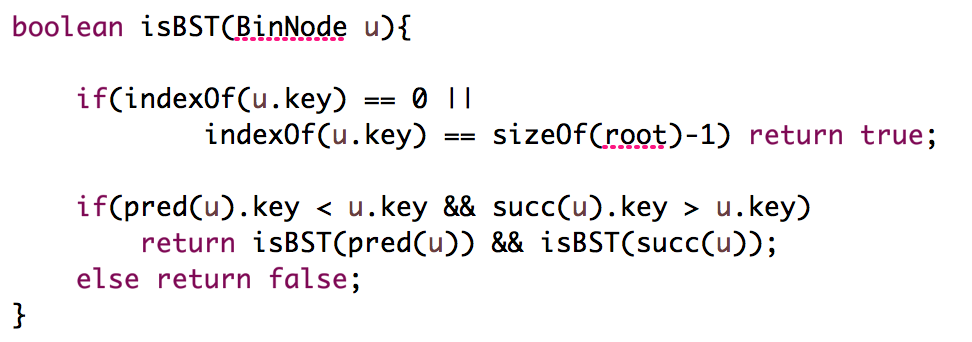
\includegraphics[width=0.8\textwidth, inner]{HW7Fig2}
		\end{figure}
		\begin{figure}[b]
			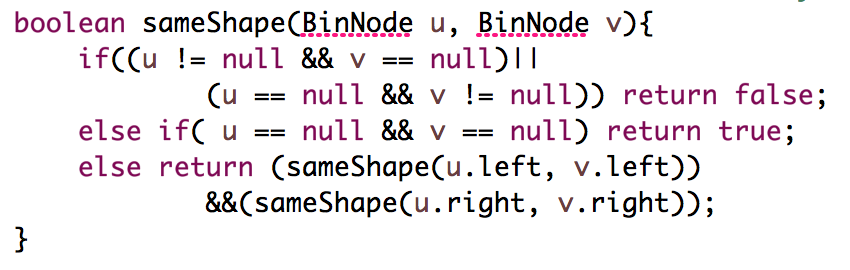
\includegraphics[width=0.7\textwidth, inner]{HW7Fig3}
		\end{figure}





\end{document}


